
\begin{frame}{The basic problem}

%\adjincludegraphics[width=0.9\textwidth,trim={0 {.5\height} 0 0 }, clip]{static_figures/survey_and_voting.jpg}

We have a survey population, for whom we observe:
%
\begin{itemize}
 \item Covariates $\x$ (e.g.~race, gender, zip code, age, education level)
 \item Responses $\y$ (e.g.~A binary response to ``do you support Trump'')
\end{itemize}
%

We want the average response in a target population,
in which we observe only covariates.


\splitpage{
    \centering
    \only<1>{
    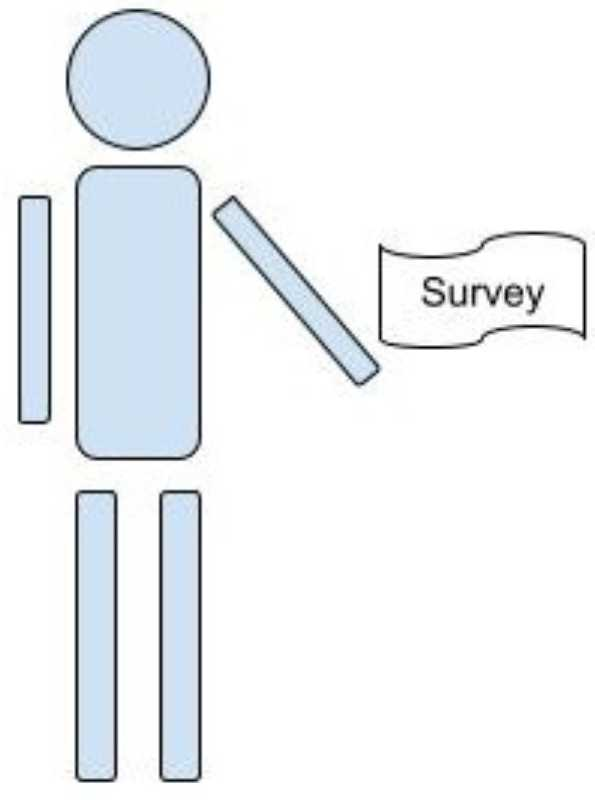
\includegraphics[width=0.5\textwidth]{static_figures/survey_man.jpg}
    }
    \only<2->{
    
\includegraphics[width=0.5\textwidth]{static_figures/survey_crazy_man.jpg}
    }
}{
    \centering
    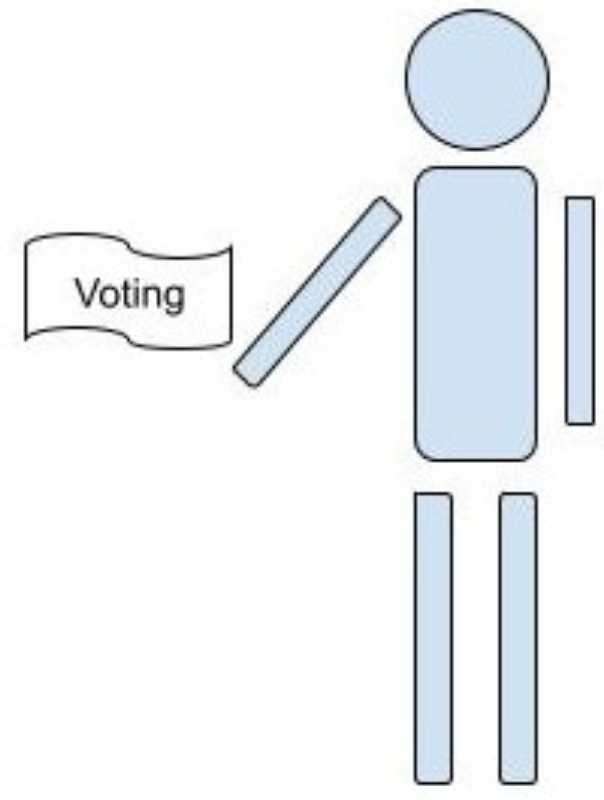
\includegraphics[width=0.5\textwidth]{static_figures/voting_man.jpg}
}

\splitpage{
    \centering
    Observe \surcol{$(\x_i, y_i)$ for $i = 1, \ldots, \nsur$}\\
}{
    \centering
    Observe \tarcol{$\x_j$ for $j = 1, \ldots, \ntar$}\\
}

\onslide<2->{
\textbf{The problem is that the populations may be very different.}
}

\onslide<3->{
    Our survey results may be biased.

    How can we use the covariates
    to say something about the target responses?
}
%
\end{frame}

%%%%%%%%%%%%%%%%%%%%%%%%%%%%%%%%%%%%%%%%%%%%%%%%%%%%%%%
%%%%%%%%%%%%%%%%%%%%%%%%%%%%%%%%%%%%%%%%%%%%%%%%%%%%%%%
%%%%%%%%%%%%%%%%%%%%%%%%%%%%%%%%%%%%%%%%%%%%%%%%%%%%%%%

\begin{frame}[t]{Two approaches}

We want $\tarcol{\mu := \meantar \y_j}$,
but don't observe target population $\tarcol{\y_j}$.

\begin{itemize}
    \item Assume $p(y | \x)$ is the same in both populations,
    \item But the distribution of $\x$ may be different in the survey and target.
\end{itemize}
%
\pause

\splitpagenoline{
    \centering
    \textbf{Calibration weighting (CW)}
}{
    \centering
    %\textbf{Multilevel regression and poststratification (MrP)}
    \textbf{Bayesian hierarchical modeling (MrP)}
}
%
%\\\hrulefill\\
\\[1em]
%
\splitpagenoline{
    \centering
    $\blacktriangleright$
    Choose ``calibration weights'' \surcol{$w_i$}\\
    using only the regressors $\x$\\
    (e.g.~raking weights)
}{
    \centering
    $\blacktriangleright$
    Choose $\expect{}{\y \vert \x, \theta} = m(\theta^\trans \x)$,\\
    choose prior $\p(\theta | \Sigma) \p(\Sigma)$\\
    (e.g.~Hierarchical logistic regression)
} \pause
%
\\[1em]
\splitpagenoline{
    \centering
    $\blacktriangleright$ Take
    $\surcol{\muhat_{\cal} = \meansur w_i y_i}$
}{
    \centering
    $\blacktriangleright$ Take
    $\tarcol{\yhat_j} =
        \expect{\postsur}{\y | \tarcol{\x_j}}$ and\\
    $\surcol{\muhat_{\mrp}} = \tarcol{\meantar \yhat_j}$
}\pause
%
\\[1em]
\splitpagenoline{
    \centering
    $\blacktriangleright$ Dependence %of \surcol{$\muhat_{\cal}$}
    on \surcol{$\y_i$} is clear\\
    % (\surcol{$\w_i$} typically chosen using only $\x$)
}{
    \centering
    $\blacktriangleright$ Dependence %of \surcol{$\muhat_\mrp$}
    on \surcol{$\y_i$} very complicated\\
    (Typically via MCMC draws from $\postsur$)
}\pause
%
\\[1em]
\splitpagenoline{
    \centering
    $\blacktriangleright$ Weights give interpretable diagnostics:
    %
    \begin{itemize}
        \item Frequentist variability
        \item Partial pooling
        \item Regressor balance
    \end{itemize}
    %
}{
    \centering
    $\blacktriangleright$ \textbf{Black box}\\
    \pause
    \vspace{1em}
    $\leftarrow$ We open this box, providing analogues of all these diagnostics
}


\end{frame}


%%%%%%%%%%%%%%%%%%%%%%%%%%%%%%%%%%%%%%%%%%%%%%%%%%%%%%%
%%%%%%%%%%%%%%%%%%%%%%%%%%%%%%%%%%%%%%%%%%%%%%%%%%%%%%%
%%%%%%%%%%%%%%%%%%%%%%%%%%%%%%%%%%%%%%%%%%%%%%%%%%%%%%%

\begin{frame}{Prior work}

\textcite{gelman:2007:struggles} observes that MrP is a CW estimator when
one uses linear regression to form $\yhat$:
$$
\begin{aligned}
% \yhat_j ={}& \x_j^\trans \betahat  =
%     \x_j^\trans \left(\sumsur \x_i \x_i^\trans \right)^{-1} \sumsur \x_i \y_i \Rightarrow \\
\surcol{\muhat_{\mrp}} ={}& \tarcol{\meantar \yhat_j} =
\tarcol{\meantar }
\underbrace{\tarcol{\x_j^\trans} \surcol{\betahat}}_{\textrm{Linear in }\surcol{\y_i}}
% =
% \surcol{\sumsur}
% \underbrace{
% \left(\tarcol{\meantar \x_j^\trans}
%     \surcol{
%         \left(\sum_{i'=1}^{\Nsur} \x_{i'} \x_{i'}^\trans \right)^{-1} \x_i
%     }
% \right)
% }_{\surcol{\w^\mrp_i}}  \surcol{\y_i} \\
\end{aligned}
$$

Most existing literature on comparing CW and MrP focus on such linear models.
\footnote{
    For example,
    \textcite{gelman:2007:struggles,benmichael:2021:multilevel,chattopadhyay:2023:implied}.}

\onslide<2->{
But what if you use a non--linear link function?  Or a hierarchical model?\\
\vspace{2em}
\hrulefill
\begin{displayquote}
``It would also be desirable to use nonlinear methods  ...
but then it would seem difficult to construct
even approximately equivalent weights.  Weighting and fully nonlinear models
would seem to be completely incompatible methods.''
--- \parencite{gelman:2007:strugglesrejoinder}
\end{displayquote}
}
\vspace{1em}

Let's spend some time discussing why it is reasonable
to even attempt such a thing as forming approximate equivalent
weights for non--linear estimators.

\end{frame}





%%%%%%%%%%%%%%%%%%%%%%%%%%%%%%%%%%%%%%%%%%%%%%%%%%%%%%%
%%%%%%%%%%%%%%%%%%%%%%%%%%%%%%%%%%%%%%%%%%%%%%%%%%%%%%%
%%%%%%%%%%%%%%%%%%%%%%%%%%%%%%%%%%%%%%%%%%%%%%%%%%%%%%%

\begin{frame}[t]{Equivalent weights for (some) logistic regression MrP}

Consider logistic regression MrP:
%
\begin{itemize}
    \item Model $\m(\x^\trans \beta) = \mathrm{Logistic}(\x^\trans \beta)$
    \item Let $\betahat$ be the MLE
    \item MrP is $\muhat_\mrp = \meantar \m(\x_j^\trans \betahat)$.
\end{itemize}
%
Suppose $\x \in \mathcal{X}$ is discrete and saturated.

\textbf{Then logistic MrP is a CW estimator.}

\pause
\def\ybar{\overline{y}}
\def\Ntarc{N_T^c}
\def\Nsurc{N_S^c}
%
\begin{itemize}
    % \item Let $N_S^c$ (or $\Ntar^c$) denote the \# of survey (or target) observations with $\x_n = c$.
    % \item When $\x_n = c$, $\m(\x_j^\trans \betahat) = \frac{1}{\Nsur^c} \sumsur \y_i \ind{\x_n = c}$.
    \item Let $\ybar_S^c$ denote the survey average among $\x = c$ for $c \in \mathcal{X}$
    \item For $\x = c$, $m(\betahat^\trans \x) = \ybar_S^c$
    \item Let $\Nsurc$ (or $\Nsurc$) denote the \# of survey (or target) observations with $\x_n = c$.
\end{itemize}
%
$$
\begin{aligned}
\muhat_\mrp ={}& \meantar \m(\x_j^\trans \betahat)
            = \frac{1}{\Ntar} \sum_{c \in \mathcal{X}}
            \underbrace{\Ntarc \ybar_S^c}_{\textrm{Linear in }\y_i}
        = \meansur \w_i^\mrp \y_i
\\ \textrm{For }
\w_i^\mrp ={}&
    \frac{\Ntarc / \Ntar}{\Nsurc / \Nsur} \textrm{ when }\x_i=c.
\end{aligned}
$$

\end{frame}


%%%%%%%%%%%%%%%%%%%%%%%%%%%%%%%%%%%%%%%%%%%%%%%%%%%%%%%
%%%%%%%%%%%%%%%%%%%%%%%%%%%%%%%%%%%%%%%%%%%%%%%%%%%%%%%
%%%%%%%%%%%%%%%%%%%%%%%%%%%%%%%%%%%%%%%%%%%%%%%%%%%%%%%

\begin{frame}[t]{Nearly equivalent weights for (some) logistic regression MrP}

\def\alphav{\mathbf{\alpha}}
%
\begin{itemize}
    \item Model $\m(\x^\trans \beta) = \mathrm{Logistic}(\x^\trans \beta)$, with MLE $\betahat$.
    \item MrP is $\muhat_\mrp = \meantar \m(\x_j^\trans \betahat)$.
\end{itemize}
%
Suppose $\x \in \mathcal{X}$ is continuous, but there exists $\alphav$
such that
$\frac{\ptar(\x)}{\psur(\x)} \approx \alphav^\trans \x$.

\textbf{Then logistic MrP is approximately a CW estimator.}\pause
% The MLE satisfies
% $\meansur m(\betahat^\trans \x_i) = \meansur \y_i \x_i$.  So
$$
\begin{aligned}
\muhat_\mrp ={}& \meantar \m(\x_j^\trans \betahat) \pause
\\ \approx{}&
    \int \m(\x^\trans \betahat) \ptar(\x) d\x
    & \textrm{(Law of large numbers)} \pause
\\ ={}&
    \int \frac{\ptar(\x)}{\psur(\x)} \m(\x^\trans \betahat) \psur(\x) d\x
    & \textrm{(Multiply by $\psur(\x) / \psur(\x)$)} \pause
\\ \approx{}&
    \int \left( \alphav^\trans \x\right) \m(\x^\trans \betahat) \psur(\x) d\x
    & \textrm{(By assumption)} \pause
\\ \approx{}&
    \alphav^\trans \meansur \x_i \m(\x_i^\trans \betahat)
    & \textrm{(Law of large numbers)}\pause
\\={}&
    \alphav^\trans \meansur \x_i \y_i
    & \textrm{(Property of exponential family MLEs)}
\end{aligned}
$$


\end{frame}


%%%%%%%%%%%%%%%%%%%%%%%%%%%%%%%%%%%%%%%%%%%%%%%%%%%%%%%
%%%%%%%%%%%%%%%%%%%%%%%%%%%%%%%%%%%%%%%%%%%%%%%%%%%%%%%
%%%%%%%%%%%%%%%%%%%%%%%%%%%%%%%%%%%%%%%%%%%%%%%%%%%%%%%

\begin{frame}[t]{Nearly equivalent weights for (some) logistic regression MrP}

\def\alphav{\mathbf{\alpha}}
%
\begin{itemize}
    \item Model $\m(\x^\trans \beta) = \mathrm{Logistic}(\x^\trans \beta)$, with MLE $\betahat$.
    \item MrP is $\muhat_\mrp = \meantar \m(\x_j^\trans \betahat)$.
\end{itemize}
%
Suppose $\x \in \mathcal{X}$ is continuous, but there exists $\alphav$
such that
$\frac{\ptar(\x)}{\psur(\x)} \approx \alphav^\trans \x$.

\textbf{Then logistic MrP is approximately a CW estimator.}
$$
\begin{aligned}
\muhat_\mrp =
    \meantar \m(\x_j^\trans \betahat) ={}
    \meansur \alphav^\trans \x_i \y_i + \textrm{Small error}
\end{aligned}
$$

We don't observe $\frac{\ptar(\x)}{\psur(\x)}$, so it's hard to estimate $\alpha$
directly.

\begin{block}{Key idea (informal)}
\centering
\vspace{1em}
    If $\muhat_\mrp \approx \meansur \w_i^\mrp \y_i$ for some $\w_i^\mrp$, then
    $\frac{\partial \muhat_\mrp}{\partial \y_i} \approx \w_i^\mrp.$\\
\vspace{1em}
\end{block}


\end{frame}


%%%%%%%%%%%%%%%%%%%%%%%%%%%%%%%%%%%%%%%%%%%%%%%%%%%%%%%
%%%%%%%%%%%%%%%%%%%%%%%%%%%%%%%%%%%%%%%%%%%%%%%%%%%%%%%
%%%%%%%%%%%%%%%%%%%%%%%%%%%%%%%%%%%%%%%%%%%%%%%%%%%%%%%

\begin{frame}{The weights can look very different!}

    \centering
    Does this mean anything?  Are the differences important?

    \WeightPlot{}
\end{frame}


